\begin{figure}[t]
  	\centering
  	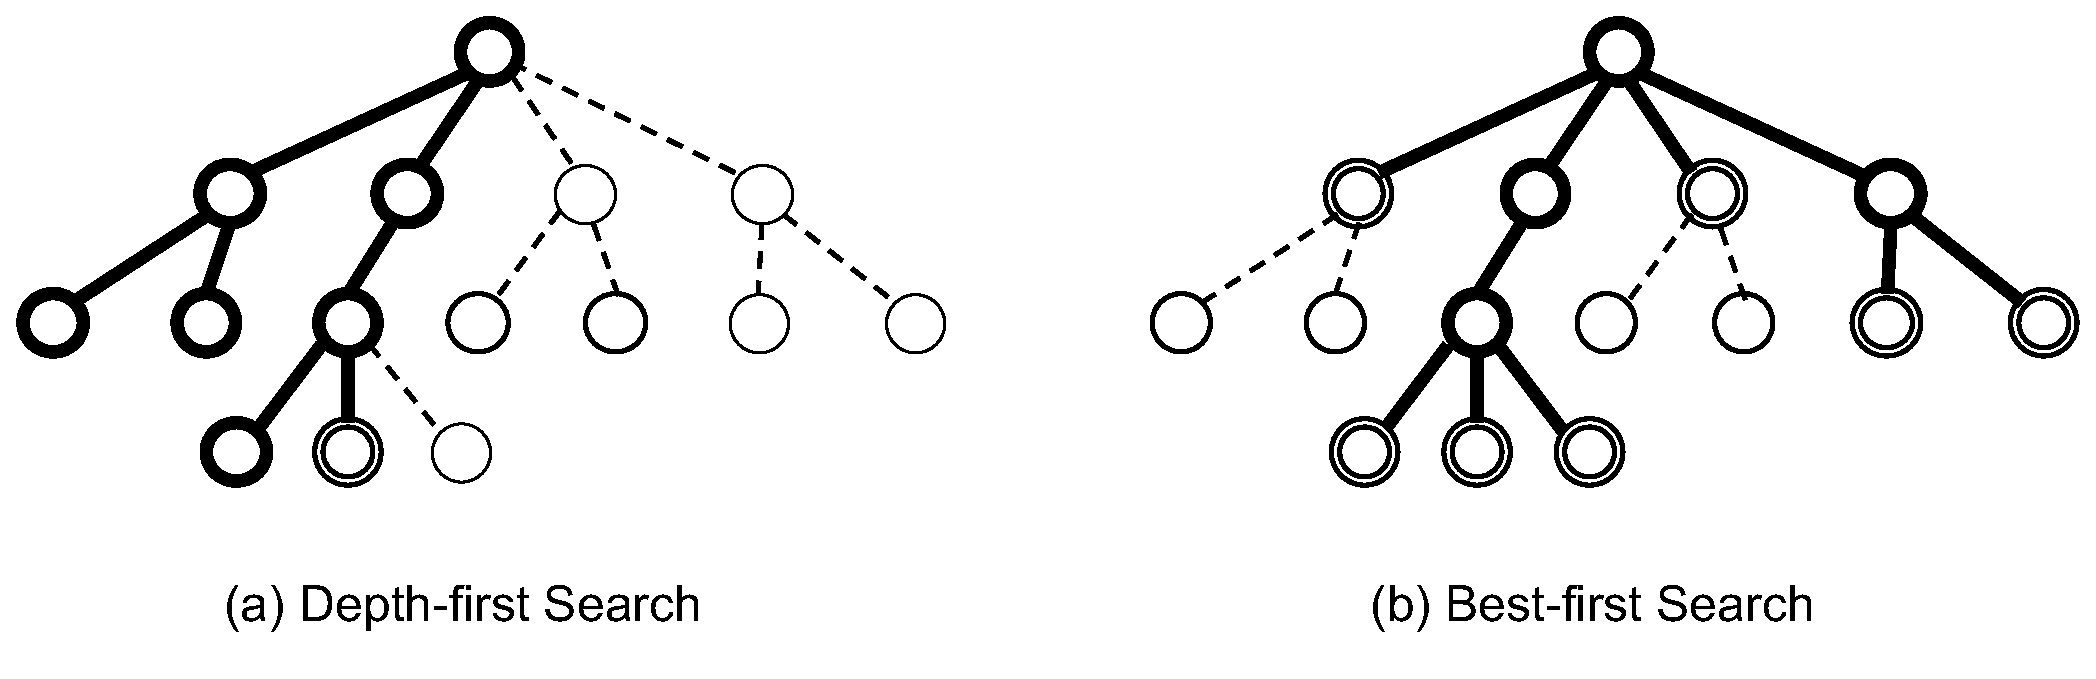
\includegraphics[width=0.9\linewidth]{img/search.eps}
	\caption{
		Where the bold circles show already searched nodes and 
		double circles show the candidate nodes for next expansion}
  	\label{fig:search}
\end{figure}

\section{Proposed Method}
The previous method employs a simple search policy with depth first
without using the discriminative criterion value ($DScore$) of each node.
In some cases, this criteria is useful for designing search policies.
In this section, using this criteria, 
we present two efficient methods to search a discriminative subgraph pattern 
based on $(i)$ Best First Search and $(ii)$ Monte Carlo Tree Search.

\subsection{Best First Search}
Best First search \cite{pearl:1984} is a search policy 
that expand from the best node based on some evaluation value, shown as Figure \ref{fig:search} (b).
The A* and Dijkstra algorithms, well known as route search algorithms, 
are also one of best first search and is known as very good search methods in some domains.

The previous method designed the pruning rule 
by calculating the bound value (\ref{eq:bound_R}). 
In the proposed method, this bound value is set as the search priority of each node, 
and is applied to the best first search.
The procedure of the proposed algorithm is illustrated with pseudocode in 
Alg.~\ref{alg:bfs}.
The search is started from the root node, 
and the node with the highest bound is selected from the expansion candidate set.
The child nodes of the selected node are expanded, 
and the score is calculated and added to the expansion candidate set.
The above operation is repeated until pruning is possible for all expansion candidate set.\\

\begin{algorithm2e}[H]
  \caption{Subgraph Search by Best First Search}
  \label{alg:bfs}
  \KwIn{Training data $\D = \{ (G_1,r_1), (G_2,r_2), \dots, (G_N,r_N) \} $}
  \KwOut{Best score subgraph $g^*$}
  \Fn{Best First Search($\D$)}{
	$candidate \leftarrow \{root\}$
    \Repeat{all candidate can be pruned}{
		$g \leftarrow \argmax_{candidate\ c} bound(c)$ \;
		$candidate \leftarrow candidate / {g}$ \;
		\ForAll{child c of g}{
      		\If{Score(c) is better than $score^*$}{
	  		  $score^*$ $\leftarrow$ $Score(c)$ \;
	  		  $g^*$ $\leftarrow$ $c$  \;
      		}
			$candidate \leftarrow candidate \cup {c}$ \;
		}
		
    }
    \KwRet{$g^*$} \;
  }
\end{algorithm2e}

\subsection{Monte Carlo Tree Search}
We consider applying Monte Carlo tree search(MCTS) 
\cite{Levente:2006, Romaric:2010, Cameron:2012} to this problem. 
MCTS is widely known as a search planning method used in computer Go, 
and is used not only as a game playing algorithm but also in various fields such as feature selection. 
One of them, Upper Confidence Bounds for Tree(UCT) algorithm 
\cite{Levente:2006} is empirically known as a way to get better solutions within a limited costs.
This method resolves the exploration-exploitation problem using Upper Confidence Bound(UCB),
which allow to estimate the expected reward of each child.
The simplest UCB policy is called UCB1 and does not require the prior specific knowledge.
The policy selects to search child node $i$ that maximizes
\begin{equation}
  \label{eq:ucb}
  UCB1 = \bar{X}_{i} + C \times \sqrt{\frac{\ln{n}}{2 n_{i}}}
\end{equation}
where $\bar{X}_{i}$ is the average reward from child node $i$, 
$n_{i}$ is the number of times child node $i$ was selected, 
$n$ is the number of times parent node of $i$ was selected,
and $C$ is an exploration constant.
The left term encourages the exploitation of high expected reward child,
and the right term encourages the exploration of less visited child.

The UCT algorithm is an iterative method 
doing the four operations of selection, expansion, 
simulation, and backpropagation up to a predefined computational cost, shown as Figure \ref{fig:MCTS}.
\begin{figure}[t]
  \centering
  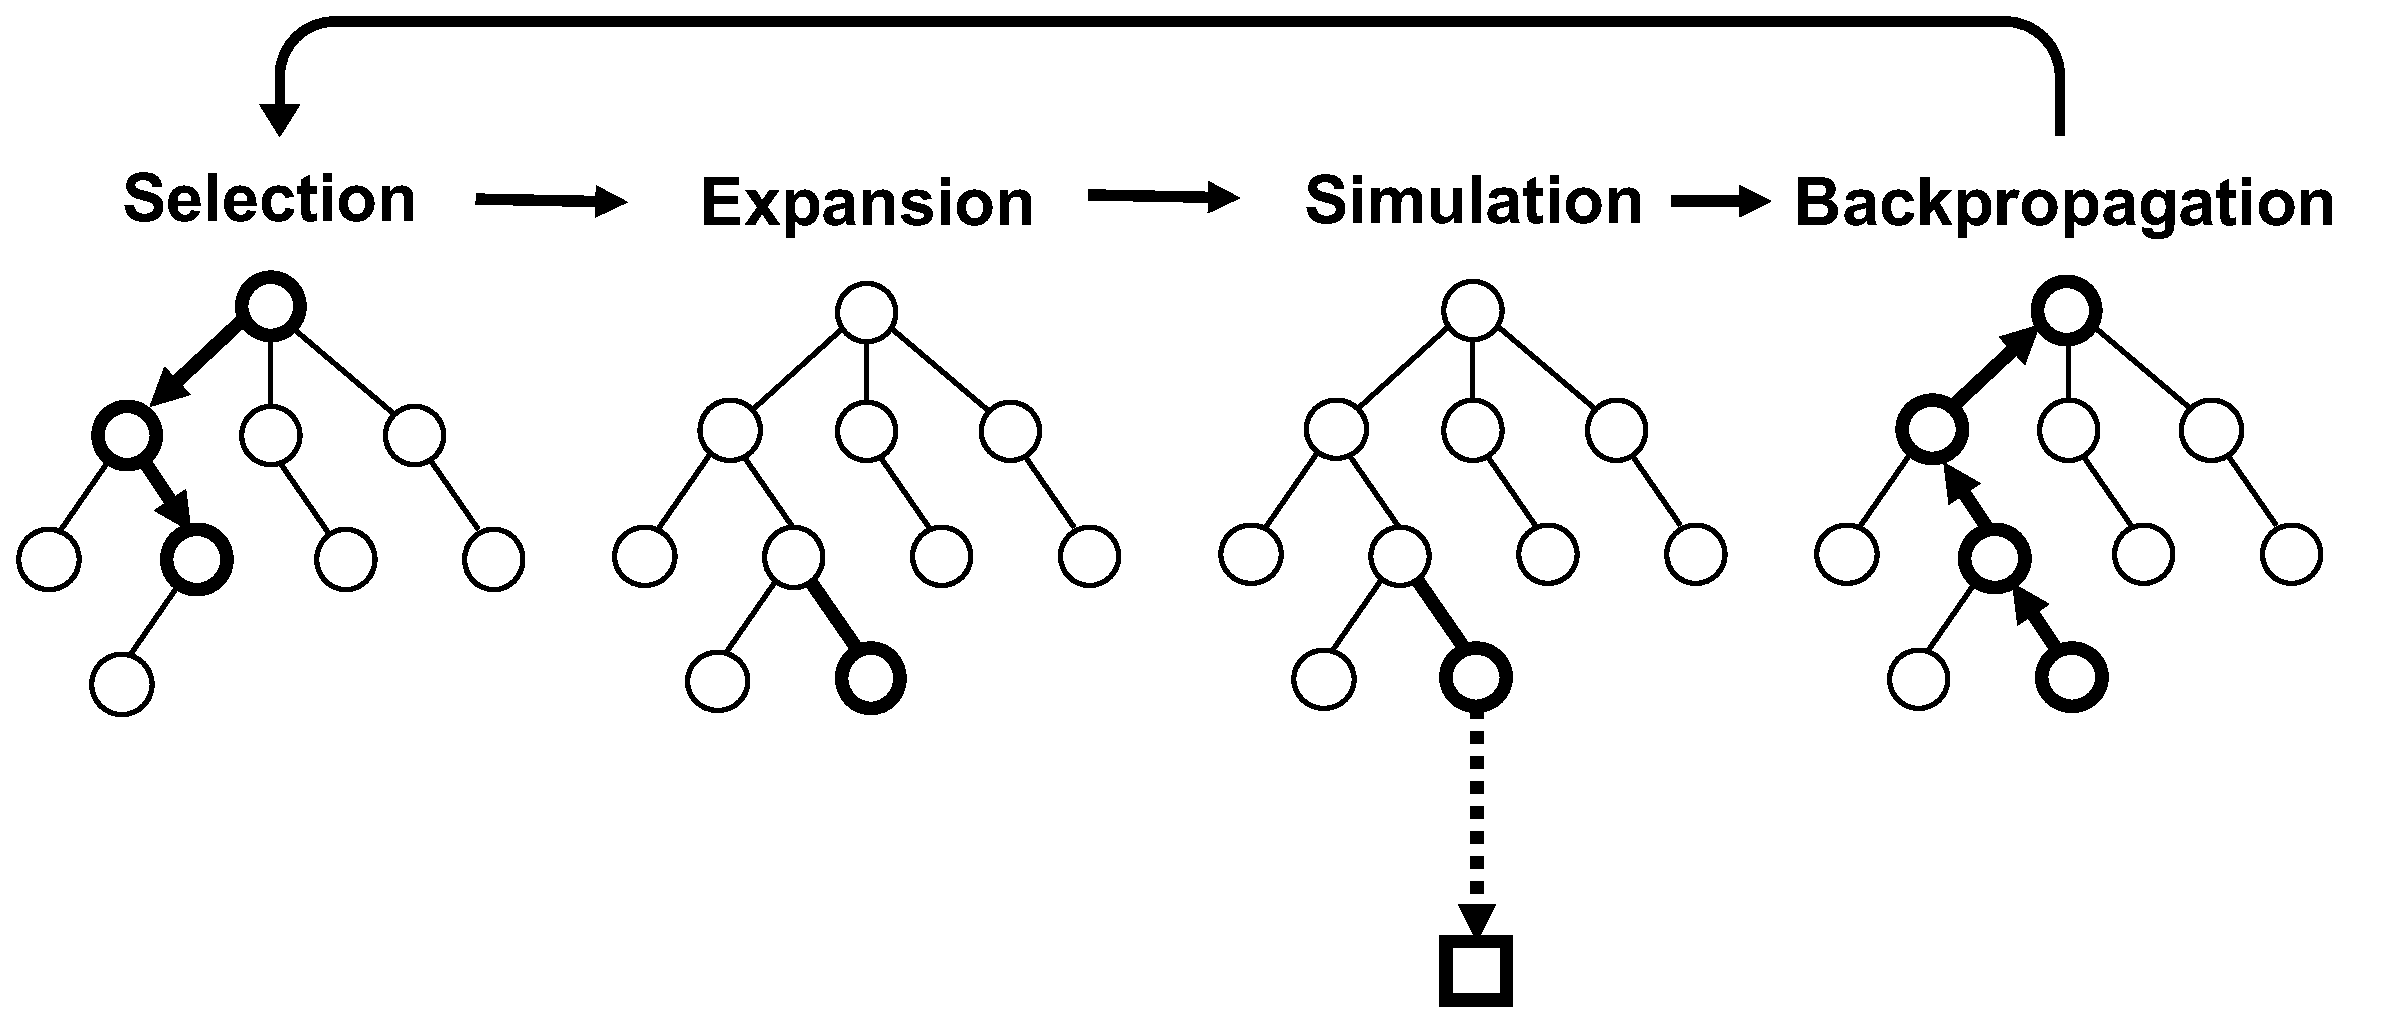
\includegraphics[width=0.9\linewidth]{img/MCTS.eps}
  \caption{One circle of processes in UCT}
  \label{fig:MCTS}
\end{figure}


\begin{enumerate}
	\item{Selection}:

	~~Start from the root node, and select the child repeatedly 
	until the expandable node is reached based on the value of (\ref{eq:ucb}).
	A node is expandable if it represents a non-terminal state and has unvisited children.

	\item{Expansion}:

	~~One random child node that is unvisited is expanded.
	In this operation, we consider the same pruning condition as (\ref{eq:bound_R}). 
	If the random select node can be pruned, another node is reselected and added.

	\item{Simulation}:
	
	~~A Monte Carlo simulation is run from the new expanded node,
	and repeatedly select a child from the available children uniformly and randomly.
	This simulation stops if the simulation node has no children or 
	is based on a stochastic condition known as a stopping feature used in \cite{Romaric:2010}.
	The stochastic condition is $1 - q^{d}$ depending on the simulation node level d,
	where $q < 1$ is a parameter and $q = 1 - 10^{-1}$ in the present paper.
	
	\item{Backpropagation}:

	~~Calculate the reward of the node $g$ obtained by simulation.
	To align the range to $[0, 1]$, reward is defined, 
	\begin{eqnarray}
		reward(g) = -DScore / \tss(\D)
	\end{eqnarray}
	these value will be large if discrimination is successful, otherwise small.
	Then backpropagate this reward to the nodes selected in selection and expansion phase.
\end{enumerate}

\subsubsection*{Low Cost Simulation}
In this problem setting, the search space is not given in advance.
Therefore, we need to construct a search space that matches the given dataset 
and subgraph search at the same time.
When Monte Carlo simulation is performed in this problem, 
it is necessary to enumerate all the child nodes for each simulation node, which requires a large cost.
We design a low-cost simulation method 
since the simulation cost has a big influence on the search efficiency.

First, a graph including simulation node is randomly selected from the dataset.
Expand the subgraph represented by the simulation node on the selected graph.
If an expanded subgraph is available(minimum order defined by \cite{Yan:2002}), 
this simulation is taken, otherwise it is repeated. \\

The entire procedure of the proposed algorithm is illustrated with pseudocode in 
Alg.~\ref{alg:uct}, \ref{alg:four_operations}.\\

\begin{algorithm2e}[H]
  \caption{Subgraph Search by UCT}
  \label{alg:uct}
  \KwIn{Training data $\D = \{ (G_1,r_1), (G_2,r_2), \dots, (G_N,r_N) \} $}
  \KwOut{Best score subgraph $g^*$}
  \Fn{UCT($\D$)}{
    \Repeat{predefined cost is exhausted}{
      \g $\leftarrow $ Selection(root) \;
      \g $\leftarrow $ Expansion(\g) \;
      \If{Score(g) is better than $score^*$}{
		$score^*$ $\leftarrow$ $Score(g)$ \;
		$g^*$ $\leftarrow$ \g  \;
      }
      $s \leftarrow $ Simulation(\g) \;
      Backpropagation($s, g$) \;
    }
    \KwRet{$g^*$} \;
  }
\end{algorithm2e}

\begin{algorithm2e}[H]
  \caption{Four Basic Operations in UCT}
  \label{alg:four_operations}
  \Fn{Selection($g$)}{
	\While{$g$ is expandable}{
		$g \leftarrow \argmax_{children\ c\ of\ g} \bar{X}_{c} + C \times \sqrt{\frac{\ln{n_{g}}}{2 n_{c}}}$ \;

	}
    \KwRet{$g$} \;
  }
  \Fn{Expansion($g$)}{
    \Repeat{g' is not pruned}{
	  $g' \leftarrow random(\{children\ c\ of\ g\})$ \;
	}
      \KwRet{$g'$} \;
  }
  \Fn{Simulation($g$)}{
	$s \leftarrow g$ \;
	\While{$s$ has some child and not enough stochastic condition}{
	  \Repeat{$s'$ is enough to minimum order}{
	  	$G \leftarrow random(\D)$ \;
	  	$s' \leftarrow random\ expansion\ from\ s\ on\ G$ \;
	  }
	  $s \leftarrow s'$ \;
	}
      \KwRet{$s$} \;
  }
  \Fn{Backpropagation($s, g$)}{
	$X = Score(s)$ \;
	\While{$g \neq NULL$}{
		$n_{g} \leftarrow n_{g} + 1$ \;
		$\bar{X}_{g} \leftarrow \frac{\bar{X}_{g} \times (n_{g} -1) + X}{n_{g}}$ \;
		$g \leftarrow parent\ of\ g$ \;
	}
  }
\end{algorithm2e}
